\section{Tổng quan quá trình Học và Giải đề ĐGNL}
\subsection{Kiến thức căn bản}\label{sec:basic}
Đối với các kiến thức căn bản, các bạn xem kĩ hơn ở phần 4: \hyperref[sec:bigbasic]{Kiến thức căn bản}
\\Các lĩnh vực chính: Tiếng Việt, Tiếng Anh, Toán, Khoa học tự nhiên, Khoa học xã hội.
\subsection{Giải đề}
\subsubsection{Lưu ý}

\paragraph{Đôi lời về bộ đề ĐGNL và việc giải đề}

\begin{itemize}
    \item Trong bộ đề gồm 20 đề - tức là rất nhiều. Mục đích của các bạn \textbf{không phải là làm hết 20 đề} này.
    \item \textbf{Bước 1:} Các bạn nên làm 1 đến 2 đề (hoặc làm đề mẫu năm 2024 \cite{demau2024}) với mục đích \textbf{tìm giới hạn  \hyperref[sec:phamvikienthuc]{phạm vi kiến thức}} mà đề sẽ hỏi. 
    \item \textbf{Bước 2:} \textbf{học và nắm chắc phần kiến thức} này.
    \item \textbf{Bước 3:} Giải đề để \textbf{nâng cao \hyperref[sec:kinanglambai]{kĩ năng}} làm bài thi. Có thể lặp lại từ bước 1.
    \item \textbf{Lưu ý:} Chỉ giải đề khi đã có lượng kiến thức căn bản nhất định (hãy nắm chắc \hyperref[sec:basic]{Kiến thức căn bản} trước). 
\end{itemize}

\subsubsection{Kĩ thuật giải đề}
\textbf{Luyện tập thông thường:} Các bạn có thể chuyển qua \hyperref[sec:giaidephongthi]{Luyện tập giải đề trong phòng thi} hoặc theo các bước sau:

\begin{enumerate}
    \item Sử dụng \href{https://www.example.com}{Bộ đề ôn thi ĐGNL} \cite{bo_de_thidgnl}
    \item \textbf{Giải đề} và đánh dấu lại đáp án.
    \item Mở đáp án của bộ đề, \textbf{chấm điểm, ghi chú} lại những kiến thức còn thiếu hoặc làm sai. 
    \item Cố gắng nâng cao thành tích trong những bộ đề sau.
\end{enumerate}
\begin{figure}[H]
    \centering
    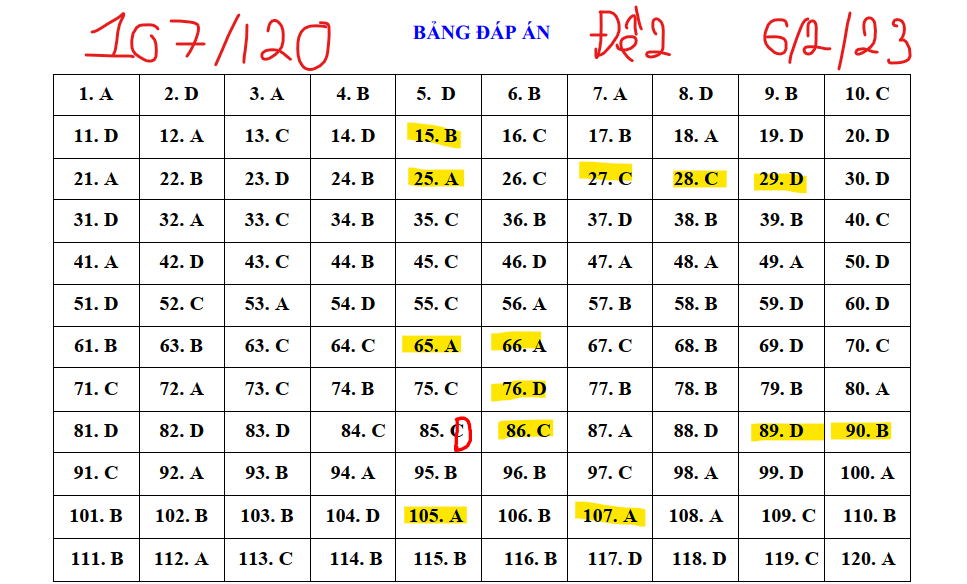
\includegraphics[width=1\linewidth]{img/Đề 2 -107_120.png}
    \caption{Đối chiếu đáp án và chấm điểm}
    \label{fig:giaidethu}
\end{figure}

\paragraph{Luyện tập giải đề trong phòng thi:}\label{sec:giaidephongthi}
\begin{enumerate}
    \item Sử dụng \href{https://www.example.com}{Bộ đề ôn thi ĐGNL} \cite{bo_de_thidgnl}
    \item Tải \href{https://drive.google.com/file/d/1IhtAQb20qTUOxD3zjC1bvKnkarBYnSok/view?usp=drive_link}{Phiếu A4 - 120 câu} \cite{phieuA4} và in trên tờ A4 (tờ trả lời trắc nghiệm).
    \item Tải app \href{https://play.google.com/store/apps/details?id=com.quiz.marker}{Chấm thi trắc nghiệm} \cite{appchamthi} \footnote{Có thể bạn chưa biết: Các thầy cô cũng dùng một ứng dụng tương tự trên điện thoại để chấm bài thi học kì (trắc nghiệm).}
    \item Mở bảng đáp án của đề sắp giải, \textbf{điền các đáp án vào phần mềm}.
    \item Cài đặt bộ đếm giờ, \textbf{reset lại não} (để quên đáp án vừa nãy nhìn) và làm bài. \textbf{Điền đáp án trực tiếp vào tờ trả lời trắc nghiệm}.
    \item Sau khi làm bài, \textbf{dùng app} để quét tờ trắc nghiệm. 
    \item \textbf{Chấm điểm, ghi chú} lại những kiến thức còn thiếu hoặc làm sai. 
    \item Cố gắng nâng cao thành tích trong những bộ đề sau.
\end{enumerate}
\begin{figure}[H]
    \centering
    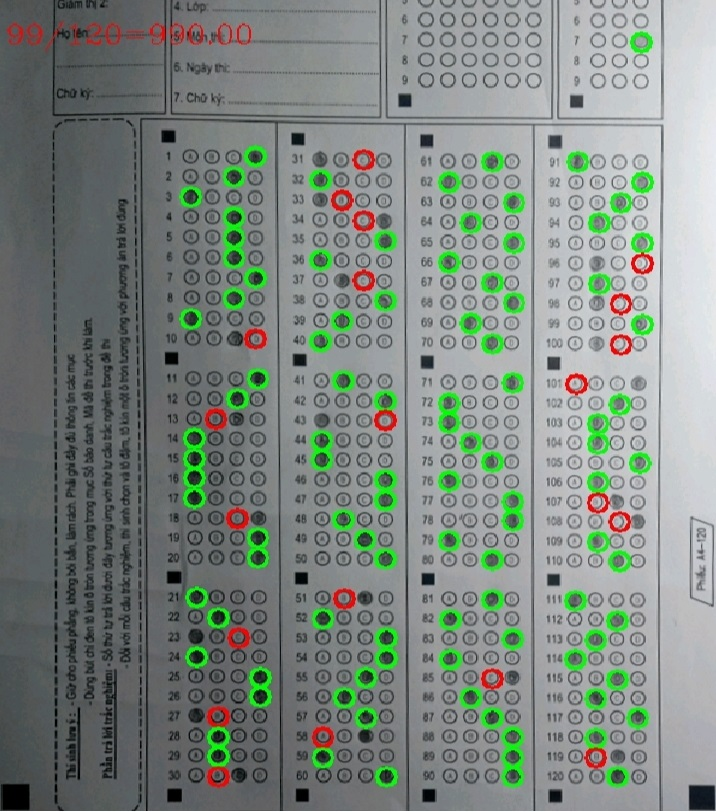
\includegraphics[width=0.7\linewidth]{img/cham_bang_app.jpg}
    \caption{Tô trắc nghiệm lên giấy và chấm bằng app}
    \label{fig:chambângppp}
\end{figure}


